\documentclass[11pt,letterpaper,boxed]{pset}

\usepackage[margin=0.75in]{geometry}
\usepackage{ulem}

\begin{document}

    \problemlist{PHYS051 HW07}
    \begin{center}
        P33.12, P33.13
    \end{center}
    
    \begin{problem} [P33.12]
    A conductor consists of an infinite number of adjacent wires, each infinitely long and carrying a current $i$. Show that the lines of $\Vec{B}$ are as represented in Fig. 33-61 and that $B$ for all points above and below the infinite current sheet is given by \[B = \frac{1}{2}\mu_0ni\]
    where $n$ is the number of wires per unit length. Derive both by direct application of Ampere's Law and by considering the problem as a limiting case of Sample Problem 33-5.
    \end{problem}
    
    \begin{figure*} [ht]
        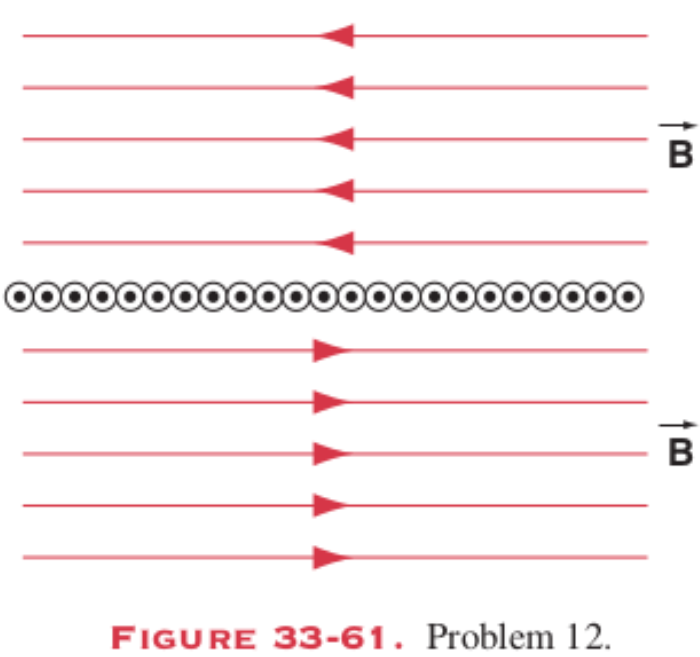
\includegraphics[width=125px]{HW7Images/P33-12.png}
        \label{fig:P33-11}
    \end{figure*}
    \newpage
    
    \begin{problem} [P33.13]
    The current density inside a long, solid, cylindrical wire of radius $a$ is in the direction of the axis and varies linearly with radial distance $r$ from the axis according to $j = j_0\frac{r}{a}$. Find the magnetic field inside the wire. Express your answer in terms of the total current $i$ carried by the wire.
    \end{problem}
    \newpage
\end{document}